\documentclass[]{article}

\usepackage[utf8x]{inputenc}
\usepackage{lmodern,textcomp}
\usepackage{lipsum}
\usepackage[margin=1in]{geometry}
\usepackage{graphicx} %Allows you to import images
\usepackage{float} %Allows for control of float positions

\usepackage{moreverb} % for verbatim ouput

% Count of words

\immediate\write18{texcount -inc -incbib 
-sum Document_Round_2_Seneka_App.tex > /Users/miequipo/Documents/wordcount.tex}
\newcommand\wordcount{
\verbatiminput{/Users/miequipo/Documents/wordcount.tex}}

% Count of characters

\immediate\write18{texcount -char -freq
 Document_Round_2_Seneka_App.tex > /Users/miequipo/Documents/charcount.tex}
\newcommand\charcount{
\verbatiminput{/Users/miequipo/Documents/charcount.tex}}


\begin{document}

\title{Seneka App\\
Universidad de los Andes\\
Airbus Fly Your Ideas}
\author{Garzón Miguel, Gómez Paula, Mendoza Santiago, Villegas Juan}
\maketitle


\Large{\textbf{1. Summary}\\}

Seneka is a platform with the ability of integrating the basic technology and engineering concepts in order to provide to the flight passengers the capacity of using their time in a pleasant way along the different airports that might be involved in their path during their business or leisure flights. Moreover, the platform brings support to the airport and airlines to allow them tracking, alerting and making contact with a passenger to notify about changes on their flight itinerary. Seneka also supports the interaction between passenger and the airport, a passenger can get notifications about the commercial offerings and the status of his order. Additionally, the passenger becomes an active member of the security team of the airport by informing to the local authorities about any emergency or misbehaviour from any other person using the app. The application has a sign-in interface for user that subsequently directs it to an airport selection interface where he or she will indicate where they want to be located and find optimal routes for their displacement. Likewise, the app has a search selection interface where the users can find stores, boarding gates and places of interest. Furthermore, an user profile interface can be found where it is possible to identify and modify their personal information and verify their flights.\\


\begin{figure}[H]
\centering
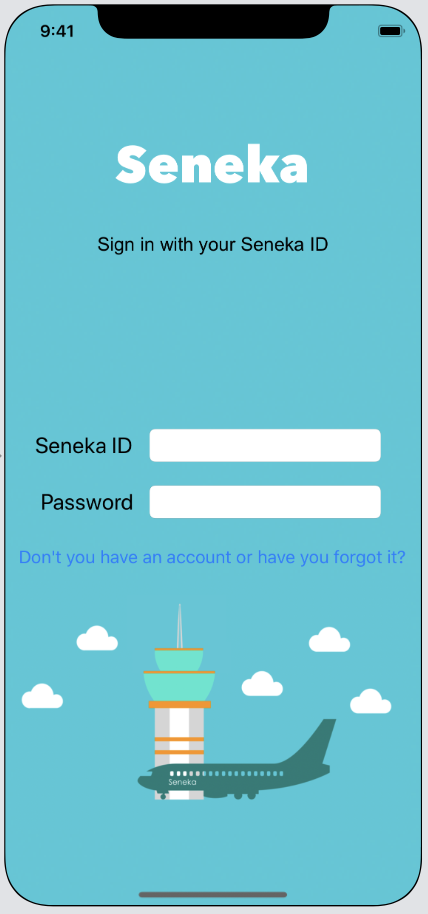
\includegraphics[height=4.0in]{Figura_1.jpg}
\end{figure}

\Large{\textbf{2. Objetives}\\}

\Large{\textbf{2.1 Main Objetive}\\}\\
[0.1cm]

Design a platform that can provide user support on his/her way through an airport by alerting, giving advice and a guidance through his/her corresponding routes within the airport, while giving secure communication channels between airports, airlines and passengers.\\
[0.7cm]

\Large{\textbf{2.2 Round 2 Specific Objetives}\\}
\begin{itemize}
	\item Design the business architecture which is consisted of the business canvas, the business ecosystem and the services brochure.
	\item Validate the acceptance of the idea throughout a market analysis based on surveys, existing companies and their success key factors.
	\item Create a functional sign-in interface based on the results of the design analysis (Colors and requirements). 
	\item Develop a broaden knowledge of the technical specifications for the mapping and location of the user.
	\item Develop a previous map interface to visualize the application on a phone.\\
[0.7cm]
\end{itemize}

\Large{\textbf{2.3 Round 3 Specific Objetives}\\}
\begin{itemize}
	\item Create a functional map interface to guide a passenger to a desired place and find commercial offers through a foreing airport.
	\item Implement a security bottom thar make the passenger connect inmediately with police or nearly security guard on the airport.
	\item Implement an "alert flight status" that gives a warning message to the passenger regarding flight status, delays and board gates updates. 
	\item Based in service brochure, we will develope an app which could be used in a cell phone with iOS system.\\
[0.6cm]
\end{itemize}

\Large{\textbf{2.4 Changes}\\}\\
Our idea has changed, from an app to a platform with the intention of provide better services to the different actors. Also, we expand our clientele, now we are creating a new form to improve the airpot traffic efficenty, making four distinct Apps for the passenger, the airport, the airlines and the shops.\\
[0.7cm]

\Large{\textbf{3. Description}\\}\\

\Large{\textbf{3.1 Development}\\}\\

In the first instance we stated the problem which consists in passengers need to locate themselves and to perform different activities in a foreign airport, as well as the airlines need for the passengers to be puntual in the boarding gates when flights are ready and the airports need of improving the traffic efficiency of people in it.\\

As an exemplification of the problem, there is a derived issue that is flights status changes such as cancellation, this affects passengers, airlines, airports and airport commerce. Specifically, when a flight is cancelled, informing passengers is currently troublesome because there is no direct communication channel between airlines and passengers, this derives in passengers losing their time by arriving the airport and find out that their flight have been cancelled, the airport gets fulled of people that are stuck waiting for another flight with a lot of baggage, airlines are one of the most affected, since the regulation EC 261 from 2004 states that any international airline has to compensate a minimum of €250 to every passenger whose flight has been cancelled in the past 3 years and hasn't been informed in the past 14 days. And this is only a special case of this lack of communication between actors in this aeronautic business of commercial travel.\\

Following this, we developed a reference architecture that allowed us to structure the IT products and services to create a solution to the stated problem, the Seneka Platform.\\
Likewise, we defined the ecosystem and the Bussiness Model Canvas of the Seneka Platform and based on those there described resources we  stablished a services catalog.\\

From the catalog services, we created a schedule in which we specified every single step that we needed to follow in the App development in accordance with the requirements that we exposed for the video.\\
[0.6cm]

\Large{\textbf{3.2 Resources}\\}\\

As first resource we implemented surveys, in order to define the most important problem for the users at the airport. Consequently,  the resources that we have used for the analysis of the data and the continuation of the process previously exposed were computers with installed software like Xcode 10, Jupiter, Atom, LaTeX and online resources like Lucidchart, GitHub, Trello and Google Forms.\\  

For the development of the video that was published in Facebook in which we showed the process of our project we used the cameras of our cellphones, images of our progress, and iMovie for the edition. Likewise, for the video that is part of the deliverables for for this round, we used images which were taken from the suggested internet webpages in the Brief document of Round 2. In addition, we counted with the help of all the staff and recoding equipment of our university to take shots and perform the edition process.\\ 


\Large{\textbf{3.3 Results, their reliability and significance}\\}\\


\Large{\textbf{3.4 Innovation}\\}\\

The aeroespace industry will get stronger as the number of passengers could feel comfortable with the security and good service. This industry, does not only rely on passengers and airlines, it also includes ground service and people working in it, that is one of the aspects that might have been forgotten or neglected. With Seneka platform and its service Seneka App, passengers, airports and airlines could be beneficiaries of the system of tracking paths within the airport, that's because people could be more in touch with all the services offered inside of it.\\

Likewise, sales will increase with the arrival of more and new travelers that are more likely to go through this airport with the revolutionary Seneka's way to buy at the airports around the world. The system is easy, the passenger selects his/her products and pays in the platform. Then enters his route and the app locates the nearest cupboard in which she/he could get the purchase without going through the airport. The cupboard are the new spaces that we identify as a pick up station, in which the seller leaves the purchase with a security code that buyer already has. Putting this code, the cupboard automatically selects the order and deliver it to the buyer in a few seconds.\\

At the same time, the congestion on hours of simultaneous boarding flights will be better as the number of travelers using Seneka App increases, because they will get an efficient path to get into the correct gate. The waiting rooms will get full only at the right times because passengers will spent their time in entertainment places without fear of losing their flights.\\

Also, as a plus for airports and passengers, Seneka will offer a service that helps clarifying the baggage opening process, in particular, Seneka will be linked with an smart lock for passengers.\\  

\Large{\textbf{4. Prototype}\\}\\

We decided that our first approach was to develop the prototype of the application in an iPhone because this kind of phones are more likely to be in the latest OS version which is an advantage while programing. In order to accomplish that we download Xcode 10, the Mac Software in which iOS apps are developed. Our main objective was to create an attractive interface while ensuring its intuitive use. To guarantee this philosophy, we based our design on Behaviorism approaches combined with the results that we obtained from the surveys. With all this information we implemented the color palette that had more acceptation and a friendly interface distribution to facilitate the use of the app. \\

\Large{\textbf{4.1 Programming process}\\}\\

We have been investigating about the scripting language Swift which is the one used for creating iOS applications in Xcode. The next stage was to start the interface design process in the computer using a powerful tool within Xcode called Storyboard. In the storyboard it is possible to drag all the required elements to properly create an app interface which are contained in what Xcode calls View Controllers (VC). We began by creating a Sign in/Log in VC with a button that takes the user to the main set of VC of the app. As we wanted to display information of multiple VC we implemented a Tab Bar at the bottom of the app interface. This allowed us to easily organize the set of 3 different buttons needed to take the user to all the 3 different interfaces of the app. These interfaces are described as Sales VC, Map VC and Profile VC. Consequently, we created Sales and Profile VC for the ones a method inside the code was used to create cells in the interface in which the different stores that are at the airport can be displayed. For the Maps VC we imported a Maps Kit to display the map and we programmed it to show the user position and to show how to get to a certain location. Finally, an Emergency VC was created to allow the user to inform or contact the local authorities within seconds. Due to this, the emergency button is located at the top right corner of all the app interface to ensure its fast location.\\

\Large{\textbf{4.2 Testing process}\\}\\

The testing of the application was at a first staged by us. Under this stage we went to El Dorado International Airport where we searched for stores with the app and then 


\Large{\textbf{5. Outcomes}\\}\\

\Large{\textbf{5.1 Achievements}\\}

The aerospace industry will get stronger as the number of passengers could feel comfortable with the security and good service. But the aerospace industry also includes ground service and people working in it, that is one of the aspects that might have been forgotten or neglected. With Seneka platform and its service Seneka App, passengers, airports and airlines could be beneficiaries of the system of tracking paths within the airport, that's because people could be more in touch with all the services offered inside of it.\\

Likewise, sales will increase with the arrival of more and new travelers that are more likely to go through this airport with the revolutionary Seneka's way to buy at the airports around the world. The system is easy, the passenger selects his/her products and pays in the platform. Then enters his route and the app locates the nearest cupboard in which she/he could get the purchase without going through the airport. The cupboard are the new spaces that we identify as a pick up station, in which the seller leaves the purchase with a security code that buyer already has. Putting this code, the cupboard automatically selects the order and deliver it to the buyer in a few seconds.\\

At the same time, the congestion on hours of simultaneous boarding flights will be better as the number of travelers using Seneka App increases, because they will get an efficient path to get into the correct gate. The waiting rooms will get full only at the right times because passengers will spent their time in entertainment places without fear of losing their flights.\\

There is also a 

\Large{\textbf{5.2 The new aerospace industry}\\}
Aquí explicamos como nuestra idea innovaría la industria y que es necesario para que sea adoptada.



\subsubsection*{Counts of words} 
\wordcount

\end{document}
